
%% bare_conf.tex
%% V1.3
%% 2007/01/11
%% by Michael Shell
%% See:
%% http://www.michaelshell.org/
%% for current contact information.
%%
%% This is a skeleton file demonstrating the use of IEEEtran.cls
%% (requires IEEEtran.cls version 1.7 or later) with an IEEE conference paper.
%%
%% Support sites:
%% http://www.michaelshell.org/tex/ieeetran/
%% http://www.ctan.org/tex-archive/macros/latex/contrib/IEEEtran/
%% and
%% http://www.ieee.org/

%%*************************************************************************
%% Legal Notice:
%% This code is offered as-is without any warranty either expressed or
%% implied; without even the implied warranty of MERCHANTABILITY or
%% FITNESS FOR A PARTICULAR PURPOSE! 
%% User assumes all risk.
%% In no event shall IEEE or any contributor to this code be liable for
%% any damages or losses, including, but not limited to, incidental,
%% consequential, or any other damages, resulting from the use or misuse
%% of any information contained here.
%%
%% All comments are the opinions of their respective authors and are not
%% necessarily endorsed by the IEEE.
%%
%% This work is distributed under the LaTeX Project Public License (LPPL)
%% ( http://www.latex-project.org/ ) version 1.3, and may be freely used,
%% distributed and modified. A copy of the LPPL, version 1.3, is included
%% in the base LaTeX documentation of all distributions of LaTeX released
%% 2003/12/01 or later.
%% Retain all contribution notices and credits.
%% ** Modified files should be clearly indicated as such, including  **
%% ** renaming them and changing author support contact information. **
%%
%% File list of work: IEEEtran.cls, IEEEtran_HOWTO.pdf, bare_adv.tex,
%%                    bare_conf.tex, bare_jrnl.tex, bare_jrnl_compsoc.tex
%%*************************************************************************

% *** Authors should verify (and, if needed, correct) their LaTeX system  ***
% *** with the testflow diagnostic prior to trusting their LaTeX platform ***
% *** with production work. IEEE's font choices can trigger bugs that do  ***
% *** not appear when using other class files.                            ***
% The testflow support page is at:
% http://www.michaelshell.org/tex/testflow/



% Note that the a4paper option is mainly intended so that authors in
% countries using A4 can easily print to A4 and see how their papers will
% look in print - the typesetting of the document will not typically be
% affected with changes in paper size (but the bottom and side margins will).
% Use the testflow package mentioned above to verify correct handling of
% both paper sizes by the user's LaTeX system.
%
% Also note that the "draftcls" or "draftclsnofoot", not "draft", option
% should be used if it is desired that the figures are to be displayed in
% draft mode.
%
\documentclass[10pt, conference, compsocconf]{IEEEtran}
% Add the compsocconf option for Computer Society conferences.
%
% If IEEEtran.cls has not been installed into the LaTeX system files,
% manually specify the path to it like:
% \documentclass[conference]{../sty/IEEEtran}





% Some very useful LaTeX packages include:
% (uncomment the ones you want to load)


% *** MISC UTILITY PACKAGES ***
%
%\usepackage{ifpdf}
% Heiko Oberdiek's ifpdf.sty is very useful if you need conditional
% compilation based on whether the output is pdf or dvi.
% usage:
% \ifpdf
%   % pdf code
% \else
%   % dvi code
% \fi
% The latest version of ifpdf.sty can be obtained from:
% http://www.ctan.org/tex-archive/macros/latex/contrib/oberdiek/
% Also, note that IEEEtran.cls V1.7 and later provides a builtin
% \ifCLASSINFOpdf conditional that works the same way.
% When switching from latex to pdflatex and vice-versa, the compiler may
% have to be run twice to clear warning/error messages.






% *** CITATION PACKAGES ***
%
%\usepackage{cite}
% cite.sty was written by Donald Arseneau
% V1.6 and later of IEEEtran pre-defines the format of the cite.sty package
% \cite{} output to follow that of IEEE. Loading the cite package will
% result in citation numbers being automatically sorted and properly
% "compressed/ranged". e.g., [1], [9], [2], [7], [5], [6] without using
% cite.sty will become [1], [2], [5]--[7], [9] using cite.sty. cite.sty's
% \cite will automatically add leading space, if needed. Use cite.sty's
% noadjust option (cite.sty V3.8 and later) if you want to turn this off.
% cite.sty is already installed on most LaTeX systems. Be sure and use
% version 4.0 (2003-05-27) and later if using hyperref.sty. cite.sty does
% not currently provide for hyperlinked citations.
% The latest version can be obtained at:
% http://www.ctan.org/tex-archive/macros/latex/contrib/cite/
% The documentation is contained in the cite.sty file itself.






% *** GRAPHICS RELATED PACKAGES ***
%
\ifCLASSINFOpdf
  % \usepackage[pdftex]{graphicx}
  % declare the path(s) where your graphic files are
  % \graphicspath{{../pdf/}{../jpeg/}}
  % and their extensions so you won't have to specify these with
  % every instance of \includegraphics
  % \DeclareGraphicsExtensions{.pdf,.jpeg,.png}
\else
  % or other class option (dvipsone, dvipdf, if not using dvips). graphicx
  % will default to the driver specified in the system graphics.cfg if no
  % driver is specified.
  % \usepackage[dvips]{graphicx}
  % declare the path(s) where your graphic files are
  % \graphicspath{{../eps/}}
  % and their extensions so you won't have to specify these with
  % every instance of \includegraphics
  % \DeclareGraphicsExtensions{.eps}
\fi
% graphicx was written by David Carlisle and Sebastian Rahtz. It is
% required if you want graphics, photos, etc. graphicx.sty is already
% installed on most LaTeX systems. The latest version and documentation can
% be obtained at: 
% http://www.ctan.org/tex-archive/macros/latex/required/graphics/
% Another good source of documentation is "Using Imported Graphics in
% LaTeX2e" by Keith Reckdahl which can be found as epslatex.ps or
% epslatex.pdf at: http://www.ctan.org/tex-archive/info/
%
% latex, and pdflatex in dvi mode, support graphics in encapsulated
% postscript (.eps) format. pdflatex in pdf mode supports graphics
% in .pdf, .jpeg, .png and .mps (metapost) formats. Users should ensure
% that all non-photo figures use a vector format (.eps, .pdf, .mps) and
% not a bitmapped formats (.jpeg, .png). IEEE frowns on bitmapped formats
% which can result in "jaggedy"/blurry rendering of lines and letters as
% well as large increases in file sizes.
%
% You can find documentation about the pdfTeX application at:
% http://www.tug.org/applications/pdftex





% *** MATH PACKAGES ***
%
%\usepackage[cmex10]{amsmath}
% A popular package from the American Mathematical Society that provides
% many useful and powerful commands for dealing with mathematics. If using
% it, be sure to load this package with the cmex10 option to ensure that
% only type 1 fonts will utilized at all point sizes. Without this option,
% it is possible that some math symbols, particularly those within
% footnotes, will be rendered in bitmap form which will result in a
% document that can not be IEEE Xplore compliant!
%
% Also, note that the amsmath package sets \interdisplaylinepenalty to 10000
% thus preventing page breaks from occurring within multiline equations. Use:
%\interdisplaylinepenalty=2500
% after loading amsmath to restore such page breaks as IEEEtran.cls normally
% does. amsmath.sty is already installed on most LaTeX systems. The latest
% version and documentation can be obtained at:
% http://www.ctan.org/tex-archive/macros/latex/required/amslatex/math/





% *** SPECIALIZED LIST PACKAGES ***
%
%\usepackage{algorithmic}
% algorithmic.sty was written by Peter Williams and Rogerio Brito.
% This package provides an algorithmic environment fo describing algorithms.
% You can use the algorithmic environment in-text or within a figure
% environment to provide for a floating algorithm. Do NOT use the algorithm
% floating environment provided by algorithm.sty (by the same authors) or
% algorithm2e.sty (by Christophe Fiorio) as IEEE does not use dedicated
% algorithm float types and packages that provide these will not provide
% correct IEEE style captions. The latest version and documentation of
% algorithmic.sty can be obtained at:
% http://www.ctan.org/tex-archive/macros/latex/contrib/algorithms/
% There is also a support site at:
% http://algorithms.berlios.de/index.html
% Also of interest may be the (relatively newer and more customizable)
% algorithmicx.sty package by Szasz Janos:
% http://www.ctan.org/tex-archive/macros/latex/contrib/algorithmicx/




% *** ALIGNMENT PACKAGES ***
%
%\usepackage{array}
% Frank Mittelbach's and David Carlisle's array.sty patches and improves
% the standard LaTeX2e array and tabular environments to provide better
% appearance and additional user controls. As the default LaTeX2e table
% generation code is lacking to the point of almost being broken with
% respect to the quality of the end results, all users are strongly
% advised to use an enhanced (at the very least that provided by array.sty)
% set of table tools. array.sty is already installed on most systems. The
% latest version and documentation can be obtained at:
% http://www.ctan.org/tex-archive/macros/latex/required/tools/


%\usepackage{mdwmath}
%\usepackage{mdwtab}
% Also highly recommended is Mark Wooding's extremely powerful MDW tools,
% especially mdwmath.sty and mdwtab.sty which are used to format equations
% and tables, respectively. The MDWtools set is already installed on most
% LaTeX systems. The lastest version and documentation is available at:
% http://www.ctan.org/tex-archive/macros/latex/contrib/mdwtools/


% IEEEtran contains the IEEEeqnarray family of commands that can be used to
% generate multiline equations as well as matrices, tables, etc., of high
% quality.


%\usepackage{eqparbox}
% Also of notable interest is Scott Pakin's eqparbox package for creating
% (automatically sized) equal width boxes - aka "natural width parboxes".
% Available at:
% http://www.ctan.org/tex-archive/macros/latex/contrib/eqparbox/





% *** SUBFIGURE PACKAGES ***
%\usepackage[tight,footnotesize]{subfigure}
% subfigure.sty was written by Steven Douglas Cochran. This package makes it
% easy to put subfigures in your figures. e.g., "Figure 1a and 1b". For IEEE
% work, it is a good idea to load it with the tight package option to reduce
% the amount of white space around the subfigures. subfigure.sty is already
% installed on most LaTeX systems. The latest version and documentation can
% be obtained at:
% http://www.ctan.org/tex-archive/obsolete/macros/latex/contrib/subfigure/
% subfigure.sty has been superceeded by subfig.sty.



%\usepackage[caption=false]{caption}
%\usepackage[font=footnotesize]{subfig}
% subfig.sty, also written by Steven Douglas Cochran, is the modern
% replacement for subfigure.sty. However, subfig.sty requires and
% automatically loads Axel Sommerfeldt's caption.sty which will override
% IEEEtran.cls handling of captions and this will result in nonIEEE style
% figure/table captions. To prevent this problem, be sure and preload
% caption.sty with its "caption=false" package option. This is will preserve
% IEEEtran.cls handing of captions. Version 1.3 (2005/06/28) and later 
% (recommended due to many improvements over 1.2) of subfig.sty supports
% the caption=false option directly:
\usepackage[caption=false,font=footnotesize]{subfig}
%
% The latest version and documentation can be obtained at:
% http://www.ctan.org/tex-archive/macros/latex/contrib/subfig/
% The latest version and documentation of caption.sty can be obtained at:
% http://www.ctan.org/tex-archive/macros/latex/contrib/caption/




% *** FLOAT PACKAGES ***
%
%\usepackage{fixltx2e}
% fixltx2e, the successor to the earlier fix2col.sty, was written by
% Frank Mittelbach and David Carlisle. This package corrects a few problems
% in the LaTeX2e kernel, the most notable of which is that in current
% LaTeX2e releases, the ordering of single and double column floats is not
% guaranteed to be preserved. Thus, an unpatched LaTeX2e can allow a
% single column figure to be placed prior to an earlier double column
% figure. The latest version and documentation can be found at:
% http://www.ctan.org/tex-archive/macros/latex/base/



%\usepackage{stfloats}
% stfloats.sty was written by Sigitas Tolusis. This package gives LaTeX2e
% the ability to do double column floats at the bottom of the page as well
% as the top. (e.g., "\begin{figure*}[!b]" is not normally possible in
% LaTeX2e). It also provides a command:
%\fnbelowfloat
% to enable the placement of footnotes below bottom floats (the standard
% LaTeX2e kernel puts them above bottom floats). This is an invasive package
% which rewrites many portions of the LaTeX2e float routines. It may not work
% with other packages that modify the LaTeX2e float routines. The latest
% version and documentation can be obtained at:
% http://www.ctan.org/tex-archive/macros/latex/contrib/sttools/
% Documentation is contained in the stfloats.sty comments as well as in the
% presfull.pdf file. Do not use the stfloats baselinefloat ability as IEEE
% does not allow \baselineskip to stretch. Authors submitting work to the
% IEEE should note that IEEE rarely uses double column equations and
% that authors should try to avoid such use. Do not be tempted to use the
% cuted.sty or midfloat.sty packages (also by Sigitas Tolusis) as IEEE does
% not format its papers in such ways.





% *** PDF, URL AND HYPERLINK PACKAGES ***
%
%\usepackage{url}
% url.sty was written by Donald Arseneau. It provides better support for
% handling and breaking URLs. url.sty is already installed on most LaTeX
% systems. The latest version can be obtained at:
% http://www.ctan.org/tex-archive/macros/latex/contrib/misc/
% Read the url.sty source comments for usage information. Basically,
% \url{my_url_here}.





% *** Do not adjust lengths that control margins, column widths, etc. ***
% *** Do not use packages that alter fonts (such as pslatex).         ***
% There should be no need to do such things with IEEEtran.cls V1.6 and later.
% (Unless specifically asked to do so by the journal or conference you plan
% to submit to, of course. )


% correct bad hyphenation here
\hyphenation{op-tical net-works semi-conduc-tor}


% ToDo notes - useful when authors are composing the document
\usepackage[colorinlistoftodos]{todonotes}
% Among other things, it provides a 'comment' directive
\usepackage{verbatim}

\begin{document}
%
% paper title
% can use linebreaks \\ within to get better formatting as desired
\title{Utilizing Unused Resources To Improve Checkpoint Performance}


% author names and affiliations
% use a multiple column layout for up to two different
% affiliations

\author{
\IEEEauthorblockN{Ross G. Miller}
\IEEEauthorblockA{Oak Ridge Leadership Computing Facility\\
Oak Ridge National Laboratory\\
Oak Ridge, Tennessee\\
Email: rgmiller@ornl.gov}
\and
\IEEEauthorblockN{E. Scott Atchley}
\IEEEauthorblockA{Oak Ridge Leadership Computing Facility\\
Oak Ridge National Laboratory\\
Oak Ridge, Tennessee\\
Email: atchleyes@ornl.gov}
}

% conference papers do not typically use \thanks and this command
% is locked out in conference mode. If really needed, such as for
% the acknowledgment of grants, issue a \IEEEoverridecommandlockouts
% after \documentclass

% for over three affiliations, or if they all won't fit within the width
% of the page, use this alternative format:
% 
%\author{\IEEEauthorblockN{Michael Shell\IEEEauthorrefmark{1},
%Homer Simpson\IEEEauthorrefmark{2},
%James Kirk\IEEEauthorrefmark{3}, 
%Montgomery Scott\IEEEauthorrefmark{3} and
%Eldon Tyrell\IEEEauthorrefmark{4}}
%\IEEEauthorblockA{\IEEEauthorrefmark{1}School of Electrical and Computer Engineering\\
%Georgia Institute of Technology,
%Atlanta, Georgia 30332--0250\\ Email: see http://www.michaelshell.org/contact.html}
%\IEEEauthorblockA{\IEEEauthorrefmark{2}Twentieth Century Fox, Springfield, USA\\
%Email: homer@thesimpsons.com}
%\IEEEauthorblockA{\IEEEauthorrefmark{3}Starfleet Academy, San Francisco, California 96678-2391\\
%Telephone: (800) 555--1212, Fax: (888) 555--1212}
%\IEEEauthorblockA{\IEEEauthorrefmark{4}Tyrell Inc., 123 Replicant Street, Los Angeles, California 90210--4321}}




% use for special paper notices
%\IEEEspecialpapernotice{(Invited Paper)}


\listoftodos
\newpage             


% make the title area
\maketitle

\todo[inline]{THIS IS A DRAFT! Make sure you search all the .tex files for any more "\textbackslash{}todo" blocks before removing this one.}



\begin{abstract}
Titan, the Cray XK7 at Oak Ridge National Laboratory, has 18,688 compute nodes. Each node consists of a 16-core AMD CPU, an NVIDIA GPU and 32GB ram. In addition, there is another 6GB of ram on each GPU card. Not all the applications that run on Titan make use of all a node's resources. For applications that are not otherwise using the GPU, this paper discusses a technique for using the GPU's ram as a large write-back cache to improve the application's file write performance.
\end{abstract}

%\begin{IEEEkeywords}
%component; formatting; style; styling;
%
%\end{IEEEkeywords}


% For peer review papers, you can put extra information on the cover
% page as needed:
% \ifCLASSOPTIONpeerreview
% \begin{center} \bfseries EDICS Category: 3-BBND \end{center}
% \fi
%
% For peerreview papers, this IEEEtran command inserts a page break and
% creates the second title. It will be ignored for other modes.
%\IEEEpeerreviewmaketitle


% Include all the .tex files for the mail paper
\section{Introduction}
\label{sec:intro}

In most HPC applications, filesystem writes typically follow a very 'bursty' pattern. That is, there will be long periods with no file output while the application is in a compute phase, followed by a period of intense output and no computation when the application writes its checkpoint or output files.  Also, at ORNL, the filesystem is a shared resource and other users will also be putting a varying load on it. This means that the performance that a user sees at any given time will likely vary dramatically.

Having a sufficiently large node-local write-back cache could improve applications' performance in two ways.  First, if the cache is large enough to hold an entire write and the individual writes are far enough apart, then the application never has to wait on the filesystem.  It can write to the cache and then resume its computations while the cache drains to the filesystem.  Secondly, write performance should be more predictable. From the application's point of view, write speed would only limited by how fast data can be copied into the cache, and since the cache is local to the node, it is not effected by outside influences.

Titan, the Cray XK7 at Oak Ridge National Laboratory, has 18,688 compute nodes. Each node consists of a 16-core AMD CPU, an NVIDIA GPU and 32GB ram. In addition, there is another 6GB of ram on each GPU card. Not surprisingly, there are applications that do not use all the resources on a compute node.

To start with, during 2014, approximately 50\% of the compute time on Titan was used on applications that did not use the GPU at all.\cite{oareport}
There may be good reasons for this.  Utilizing the GPU's requires changes to the application and it's possible the developers haven't had the time to do that.  It's also possible that the type of computations the application performs simply don't lend themselves to GPU-based acceleration.  Regardless of why, it's clear that not all applications are benefiting from the GPU.

Secondly, though AMD markets the processor as having 16 cores, it actually has only 8 floating-point units. As such, some applications that are floating-point intensive run with only 8 processes per node. This actually leaves 8 cores available so long as they primarily execute integer instructions. 

 The unused GPU memory and integer cores can be used to implement a write-back cache without taking resources away from the main application.  This paper demonstrates a technique for providing such a cache to applications.   Runs were made on Titan using a synthetic benchmark to demonstrate performance both without such a cache and with a cache that utilizes ram on the GPU card. The results show definite performance benefits.
 

\begin{comment}

Specifically, though AMD markets the processor as having 16 cores, it actually has only 8 floating-point units. As such, some applications that are floating-point intensive run with only 8 processes per node. This actually leaves 8 cores available so long as they primarily execute integer instructions. Furthermore, some applications do not make use of the GPU and thus it, and the ram attached to it, also go unused.

Since the GPU memory is accessed via the PCIe bus, it is generally not practical to use it as part of a process's main memory. Its bandwidth is too low and its latency is too high. However, when compared to filesystem performance - even a very fast parallel filesystem - accessing this memory is still very fast. Tests on Titan show that writing to GPU memory is at least eight times faster than writing to the filesystem, and considerably better than that if the filesystem is under heavy load. This suggests that using this memory as a large write-back cache for file I/O might help application runtimes significantly.

In HPC applications, most filesystem writes follow a very ?bursty? pattern. That is, there will be long periods with no file output while the application is in a compute phase, followed by a short period of intense output when the application writes its checkpoint or output files. Furthermore, at ORNL, the filesystem is a shared resource and other users will also be putting a varying load on it. This means that the performance that a user sees at any given time will likely vary dramatically.

Having a sufficiently large write-back cache would alleviate both of these problems. Assuming the cache is large enough, then the 'bursty' nature of the output pattern can be smoothed out since there will be time for the traffic to drain from the cache before the next burst arrives. Equally importantly, write performance should be more predictable. From the application's point of view, write speed is only limited by how fast data can be copied into the cache, and that is not effected by outside influences. The GPU memory and integer cores can be used to implement such a cache without taking resources away from the main application.

This paper demonstrates a technique for providing such a write-back cache to applications. We use a synthetic benchmark to demonstrate performance without such a cache, with a cache that utilizes regular system ram and with a cache that utilizes ram on the GPU card. Performance benefits and any potential trade-offs and caveats are discussed.


 
 Since the GPU memory is accessed via the PCIe bus, it is generally not practical to use it as part of a process's main memory. Its bandwidth is too low and its latency is too high. However, when compared to filesystem performance - even a very fast parallel filesystem - accessing this memory is still very fast. Tests on Titan show that writing to GPU memory is at least eight times faster than writing to the filesystem, and considerably better than that if the filesystem is under heavy load. This suggests that using this memory as a large write-back cache for file I/O might help application runtimes significantly.


\end{comment}

\section{Design And Implementation}
\label{sec:design}

\subsection{Overview}
\label{subsec:overview}
This idea was tested using a synthetic benchmark application written by the authors.  The benchmark consists of two executables: the main application which uses MPI and simulates the I/O patterns of a typical HPC application and a daemon process that is started on each compute node.  The daemon has two tasks: manage the GPU memory and copy data from GPU memory out to a file.  Note that the daemon does \emph{not} copy the data into the GPU memory; that is handled by the individual ranks of the main application.   There needs to be exactly one daemon process on each compute node regardless of how many MPI ranks are running on each node.  \footnote{Due to the limitations of aprun, starting this daemon is somewhat involved.  See section \ref{subsec:cray-specific}.}

With the daemon process running on each node, the application begins its main execution.  In this case, since it's just a synthetic 
I/O benchmark, it performs no actual computation; it simply writes a specified amount of data and then sleeps for a specified amount of time.  For these tests, the sleep time was deliberately calculated to allow enough time for the data in GPU memory to drain.
\subsection{Communication Between the Application and Daemon}
\label{subsec:comm}

Communication between the main application and the daemon happens over two different channels.  Short messages for coordination between the application and the daemon are handled using the Common Communication Interface (CCI).\cite{atchley11:cci}  Bulk data is copied to and from GPU memory using \texttt{cudaMemcpy()}.

\todo[inline]{We need to figure out how to force figure \ref{fig:communications} to display as page 2 or 3.  Right now, latex is putting it on the last page.}
\begin{figure*}[!t]
\centerline{
  \subfloat[Application sends write request message to daemon]{
    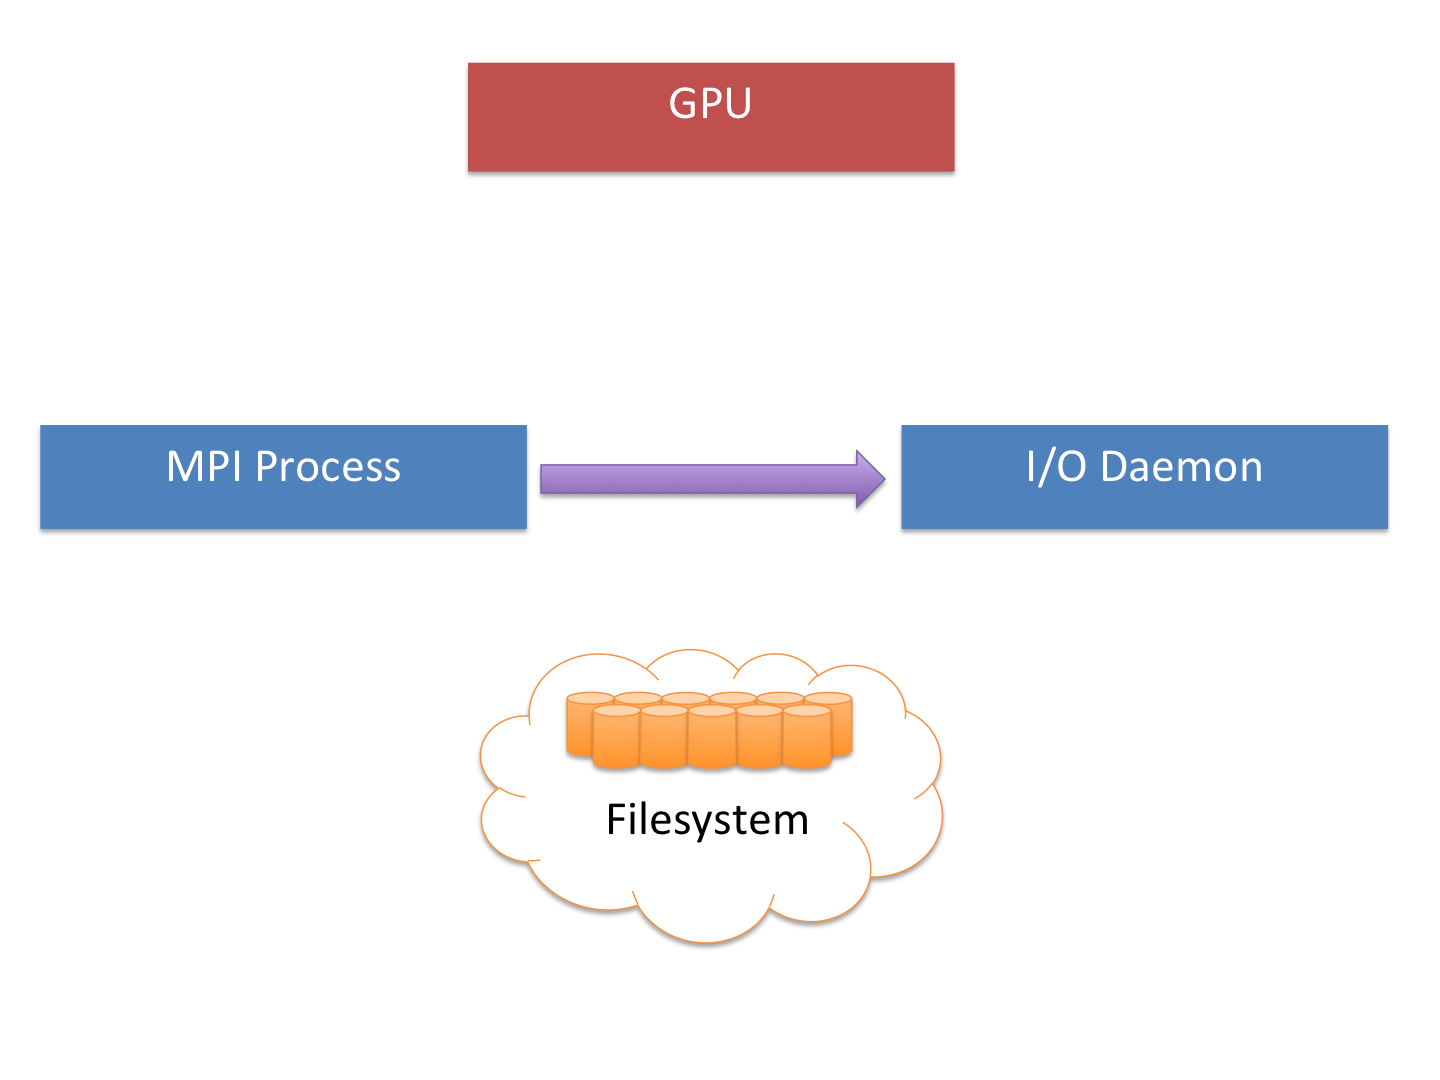
\includegraphics[width=2.5in]{figures/Data_Movement/Slide09}%
    \label{fig:comm_a}}
  \hfil
  \subfloat[Daemon allocates GPU memory and converts pointer into IPC handle]{
    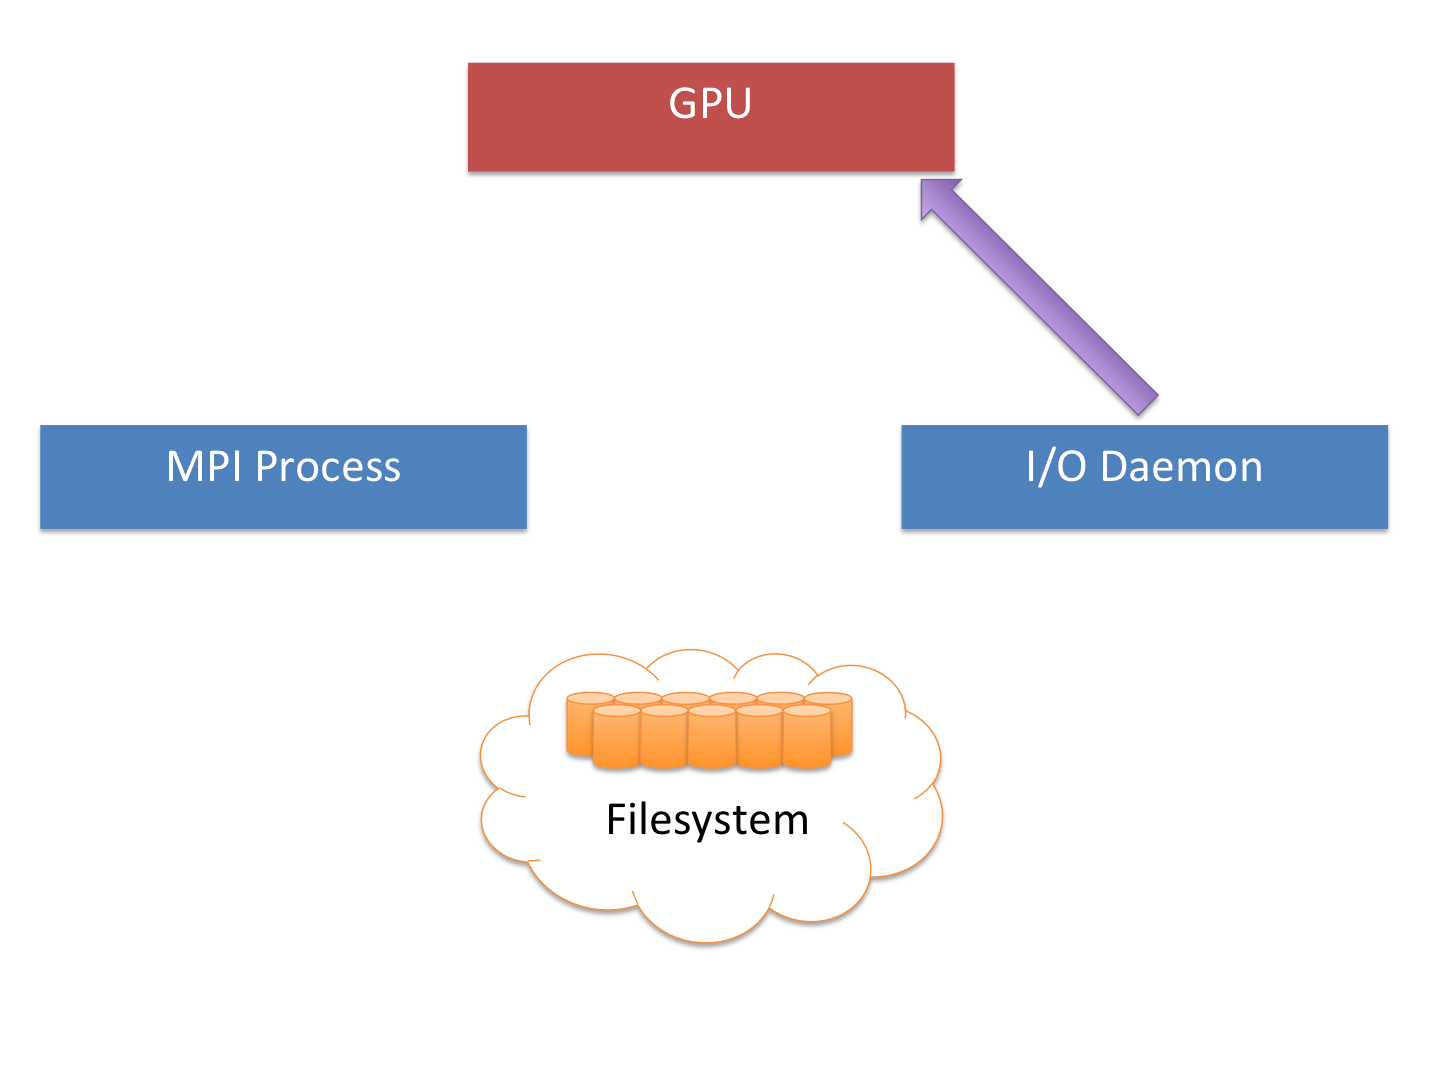
\includegraphics[width=2.5in]{figures/Data_Movement/Slide10}%
    \label{fig:comm_b}}}
\centerline{
  \subfloat[Daemon sends reply message with IPC handle]{
    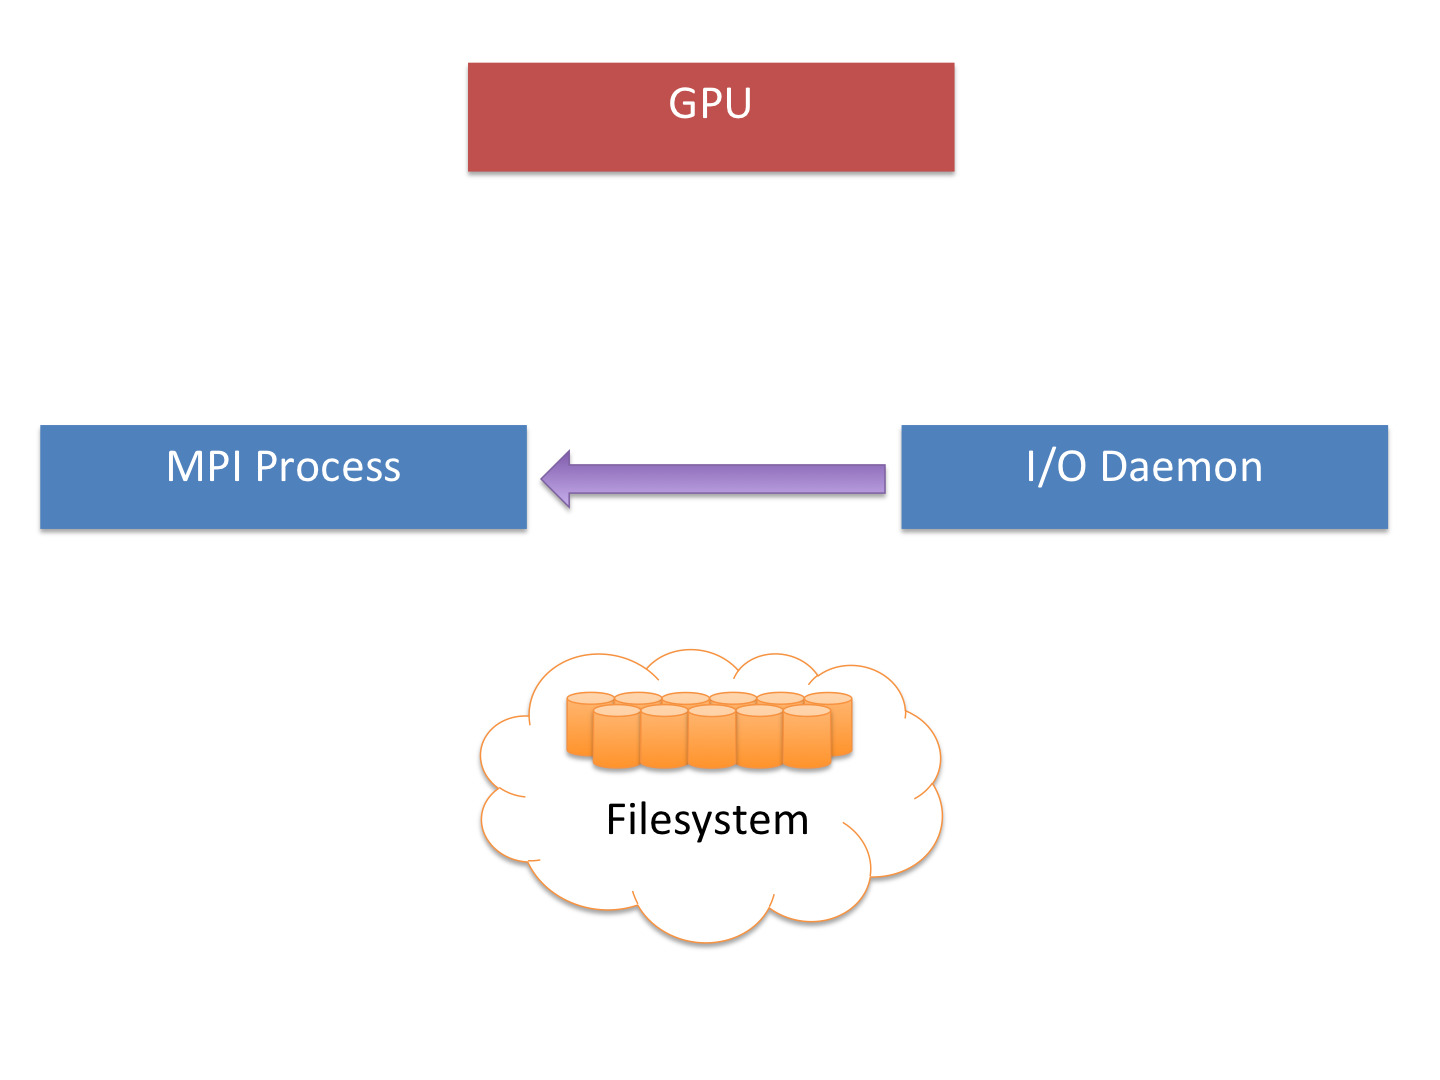
\includegraphics[width=2.5in]{figures/Data_Movement/Slide11}%
    \label{fig:comm_c}}
  \hfil
  \subfloat[Application writes data to GPU memory]{
    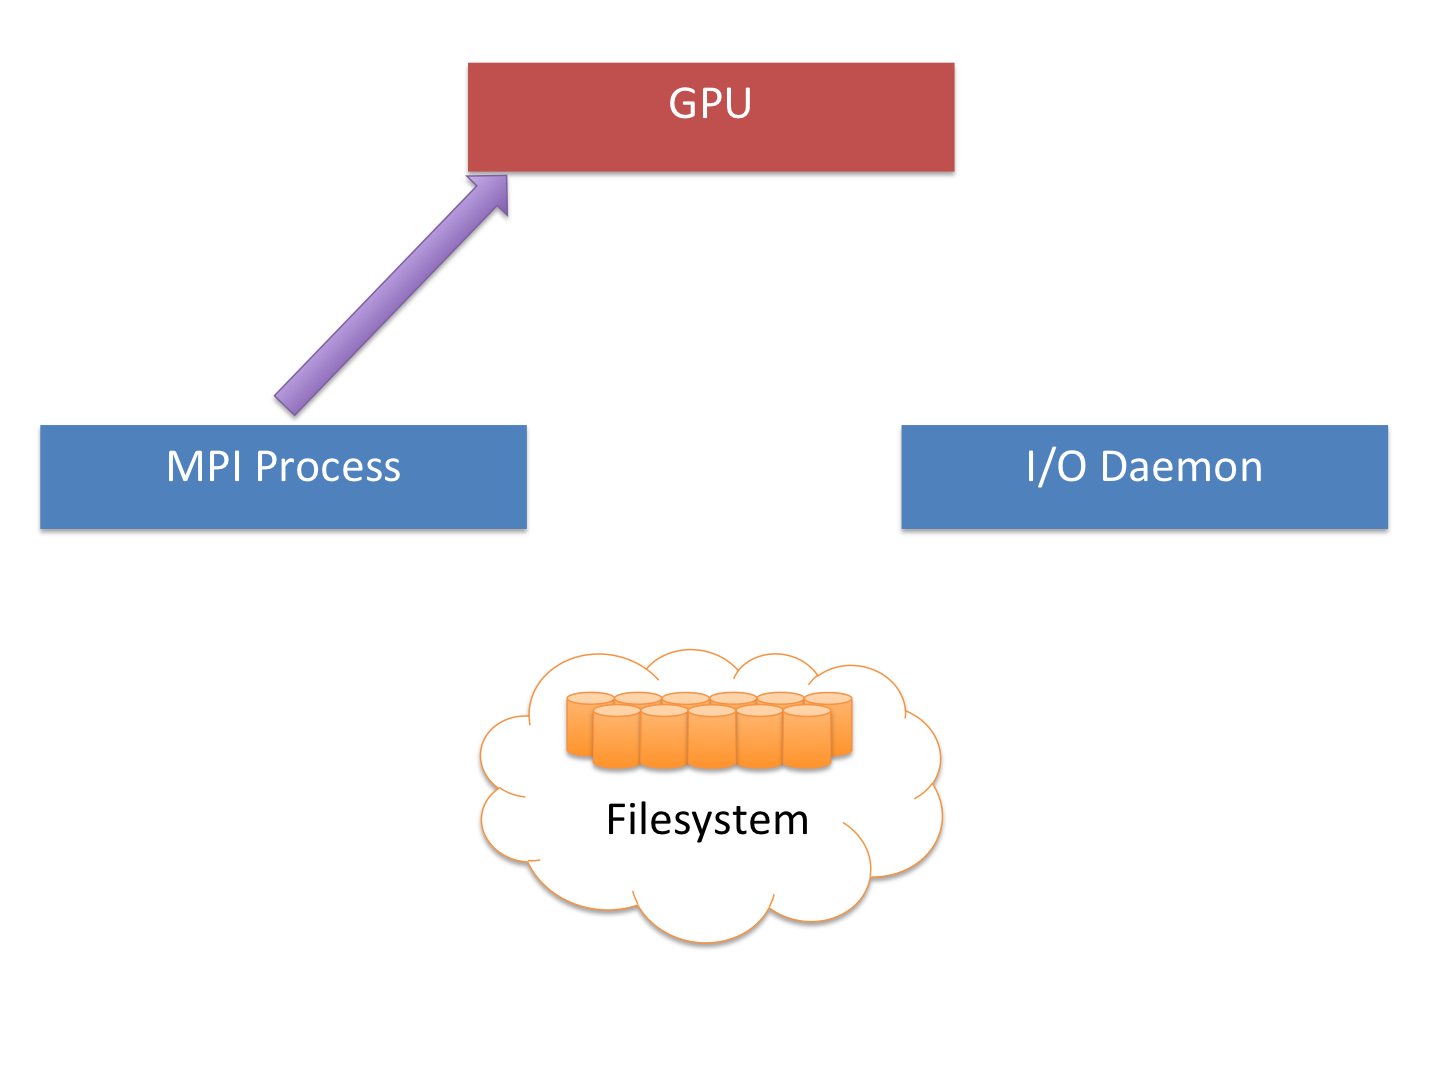
\includegraphics[width=2.5in]{figures/Data_Movement/Slide12}%
    \label{fig:comm_d}}}    
\centerline{
  \subfloat[Application sends write complete message to daemon]{
    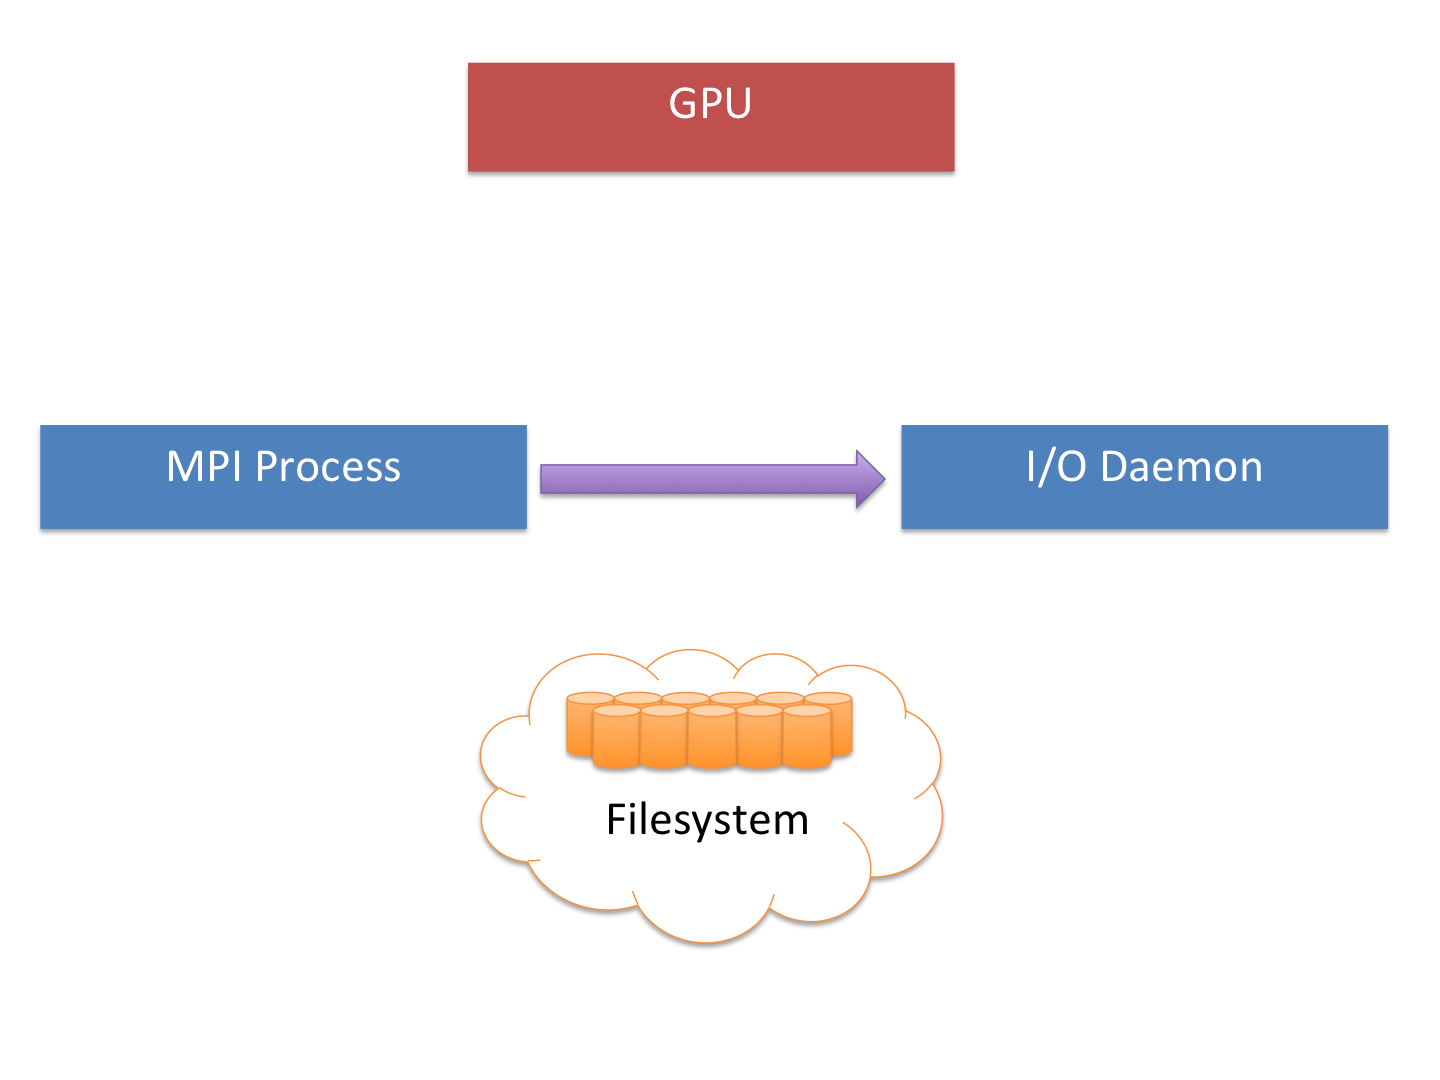
\includegraphics[width=2.5in]{figures/Data_Movement/Slide13}%
    \label{fig:comm_e}}
  \hfil
  \subfloat[Daemon copies data from GPU memory to system memory]{
    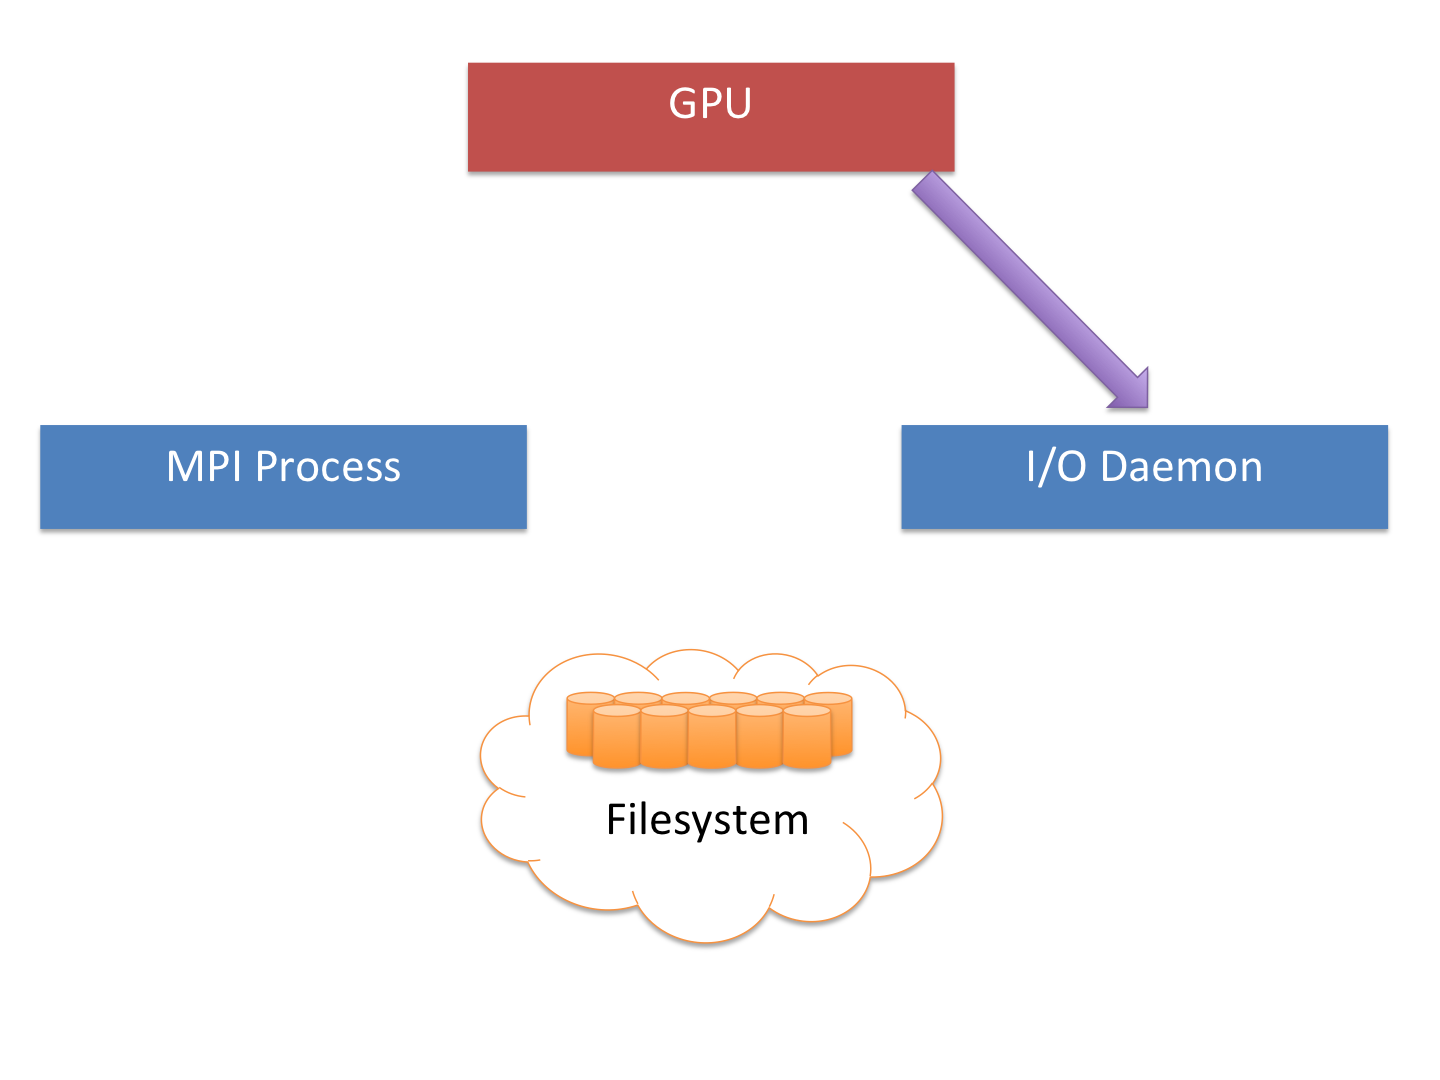
\includegraphics[width=2.5in]{figures/Data_Movement/Slide14}%
    \label{fig:comm_f}}} 
\centerline{
  \subfloat[Daemon writes data to filesystem]{
    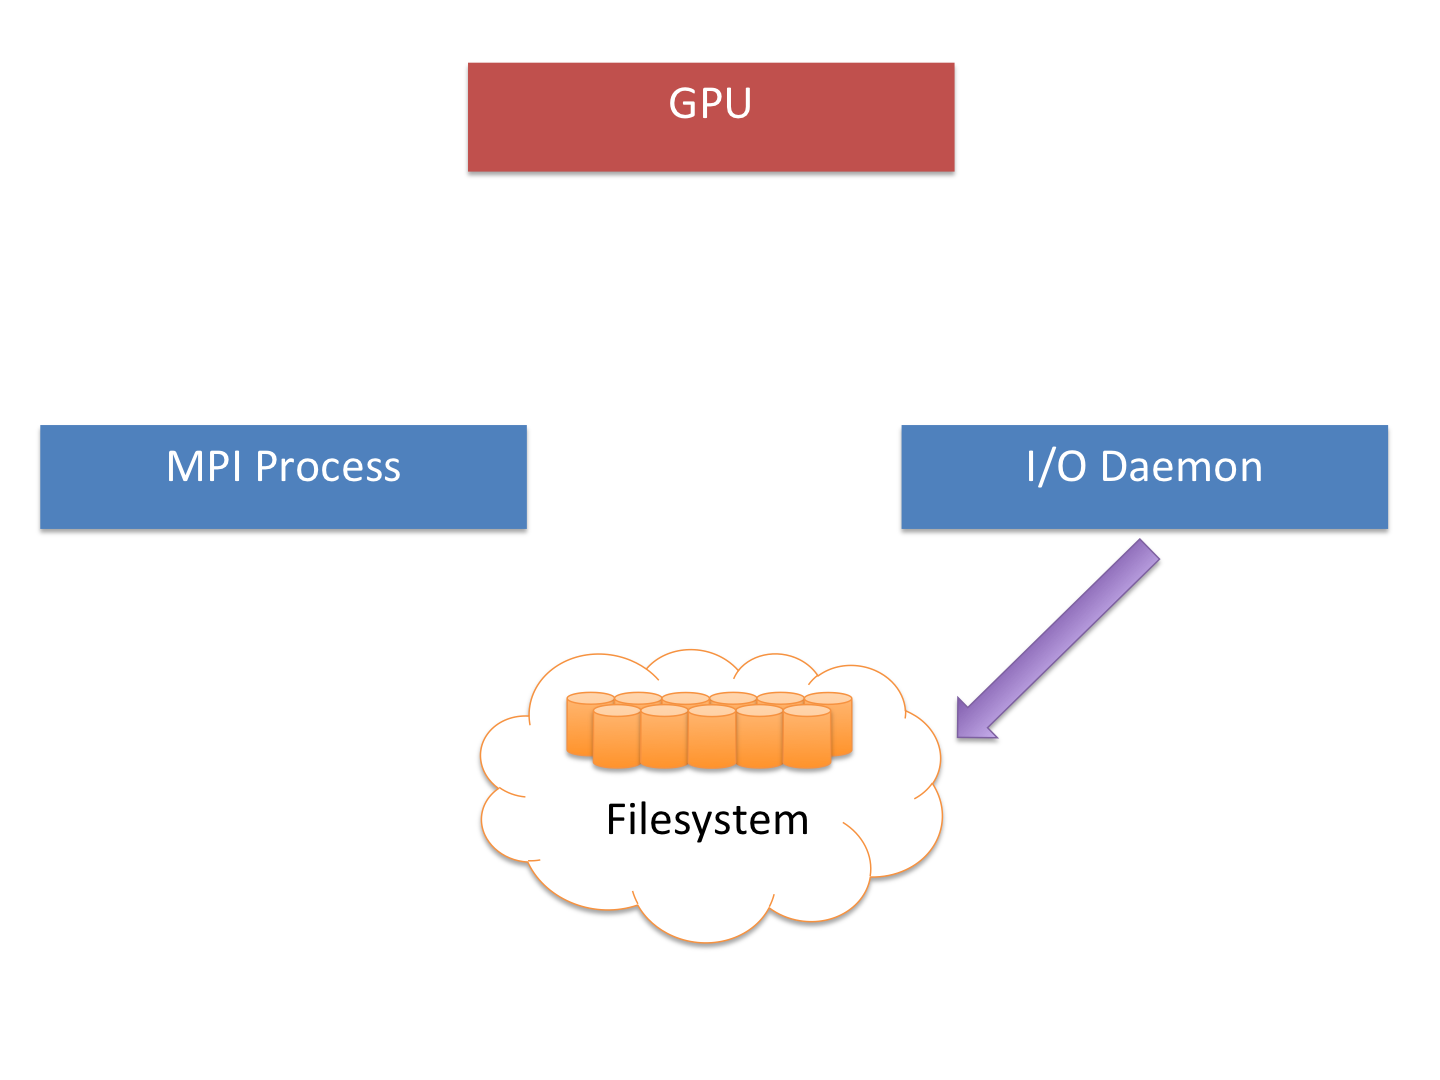
\includegraphics[width=2.5in]{figures/Data_Movement/Slide15}%
    \label{fig:comm_g}}} 
\caption{Communications steps}
\label{fig:communications}
\end{figure*}


Writing data from the application is a seven step process.

When it's time to write, the application sends a short message to the daemon using CCI.  This message is a request to write data, and contains the amount of data and the starting offset into the output file.\footnote{For this benchmark, the daemon names output files based on the MPI rank of the requestor.  For production code, something more flexible will obviously be needed.}(Figure \ref{fig:comm_a})

When the daemon receives this message, it will attempt to allocate memory on the GPU.  Assuming the allocation succeeds, the daemon will use \texttt{cudaIpcGetMemhandle()} to create a memory handle for the allocation. (Figure \ref{fig:comm_b})

The daemon will then reply to the application with the size of memory that was actually allocated and the memory handle that the application can use to access the GPU memory.  Note that the size value may be less than what the application asked for. (Figure \ref{fig:comm_c})

Upon receiving the reply, the application opens the memory handle and converts it back to a standard pointer.  The application then uses \texttt{cudaMemcpy()} to copy the specified amount of data up to the GPU memory. (Figure \ref{fig:comm_d}) 

When the copy has completed, the application closes the memory handle and sends a message back to the daemon saying that this particular write has completed.  (Figure \ref{fig:comm_e})  If the application has more data to write, it can repeat the previous steps, or else it can continue with its calculations.

Note that at this point the data has not made it out to the filesystem yet; it's just sitting in GPU memory.  

The daemon maintains a pair of lists.  One list is the blocks of GPU memory that have been assigned to the ranks of the main application, and which the ranks are presumably copying data into.  The second list is for all the blocks of memory for which the `write complete' message (step e) has been received.  When the daemon thread that handles CCI messages receives a `write done' message for a block, it moves that block from the first list to the second list.  It then notifies the background write thread(s) that the block is now ready to be written to the filesystem.

The daemon maintains one or more background threads that are responsible for copying data out of GPU memory into normal system memory and then writing that data to the filesystem.  These threads allow the writes to the filesystem to happen asynchronously while the main thread handles all the CCI messages.  Since it's impossible to write directly from GPU memory to the filesystem, each thread will copy a block of data from GPU memory into a buffer in main memory.  (Figure \ref{fig:comm_f})  It will then write the data to the output file at the location specified in the original request message.  (Figure \ref{fig:comm_g})  Once data has been written to the filesystem, the write thread free's the GPU memory so that it can be used in another request.

\begin{figure}
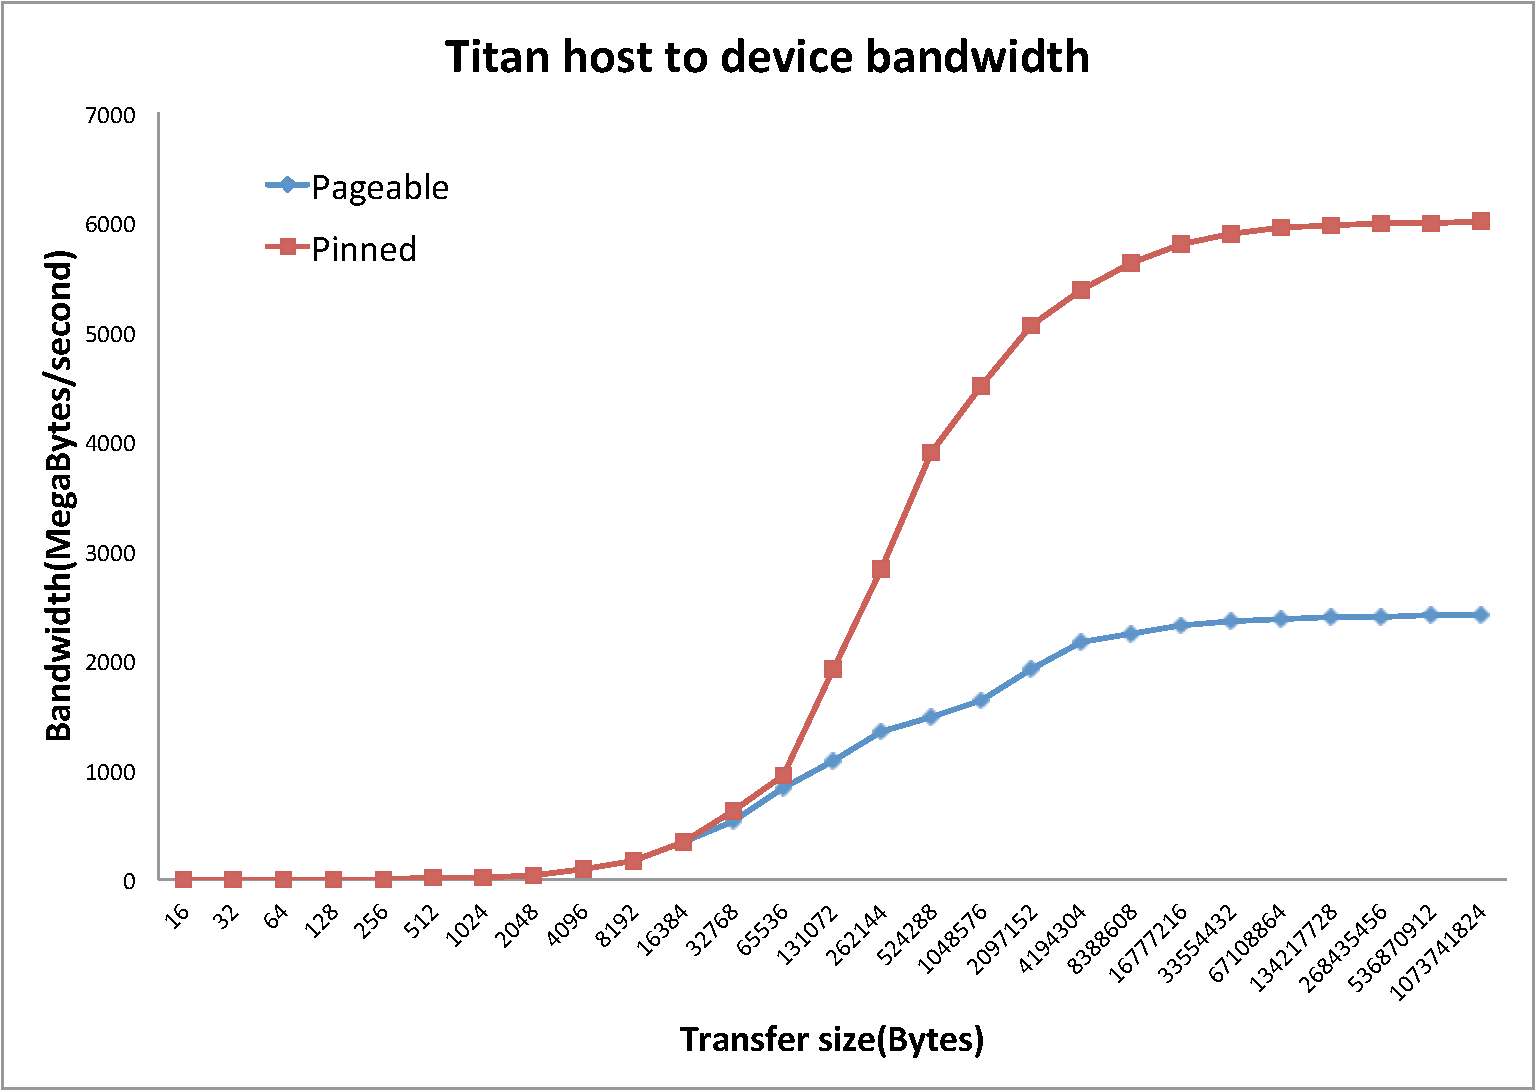
\includegraphics[width=\linewidth]{figures/Host2Device_BW.pdf}
\caption{Bandwidth between system memory and GPU memory as a function of write size\cite{ac_guide}} 
\label{fig:transfer_bw}
\end{figure}

Note that each write thread in the daemon has its own buffer in system memory.  Each of these buffers is deliberately kept fairly small - 16MB - in order to conserve resources.  Testing done on Titan shows that 16MB block sizes are large enough for \texttt{cudaMemcpy()} to give good performance.\cite{ac_guide}  Larger buffers would simply use up memory without improving performance noticeably. See Figure \ref{fig:transfer_bw}.

Also note that the daemon limits the amount of memory allocated to any single request to 16MB.  This was done to provide some limited load-balancing.  If an application wants to write 512MB, it will therefore have to make 32 separate requests.  If other ranks on the node are trying to write at the same time, their requests will all be interleaved and hopefully no rank will be starved out.


\subsection{Cray-Specific Details}
\label{subsec:cray-specific}

There are a few peculiarities of the Cray environment that need to be taken in to account in order for this software to work properly.  The first peculiarity has to do with limiting access to the GPU and associated hardware.  The CUDA runtime can be configured to limit access to the GPU to a single thread, to multiple threads from a single process or to multiple threads from multiple processes.  On Titan, if no special options are given to qsub, the CUDA runtime will be configured for a single thread.  Since software described in this paper requires access to the GPU from multiple processes, users must switch to the appropriate compute mode.  This is done by passing the flag "-l feature=gpudefault" to qsub.\footnote{It may seem strange to have to explicitly switch to a mode called 'gpudefault'.  The naming scheme comes from the CUDA documentation.  On a standard CUDA install, the GPU would in fact default to allowing access from multiple processes.  Titan is configured differently, however.  Thus the need to explicitly tell qsub to switch the GPU's to the `default' mode.}

The second peculiarity has to do with actually starting the daemon process.  Normally, executables are started on the compute nodes by aprun.  However, aprun is designed to start a single executable, not to start two different executables.  Even in MPMD mode, it won't start two different executables on the same node.  The solution is to have one rank on each node call \texttt{fork()} and then \texttt{execve()}.  Since MPI purposely hides the compute topology from the application, deciding exactly which ranks call fork() takes a little more work.  Specifically, all ranks will attempt to open a file using the \texttt{O\_CREAT} and 
\texttt{O\_EXCL} flags.  The name of the file is taken from the compute node's host name.  This combination of flags and filename ensures that exactly one rank on each node successfully opens the file.  The ranks that succeed will then start the daemon processes.

%
% Everything below is commented out.  It's text I've toyed with using, but decided not to for whatever reason
%
\begin{comment}


It's debatable whether this sort of load balancing is necessary or even desirable.  Indeed, preliminary testing seemed to indicate that it might be faster to let the daemon allocate  as much GPU memory as the client requested (assuming there was enough free).  However, that same testing showed that one of the CUDA functions - \texttt{cudaIpcOpenMemHandle()} - became unreliable once GPU memory allocations exceeded 512MB.  Until the nature of that problem could be determined, it was decided to limit allocations to 16MB.



CUDA has several functions for facilitating interprocess communications.  Among other things, one can convert a device pointer to a process-independant memory handle.  Another process can take that memory handle and convert it back to a device pointer.


\end{comment}


\section{Analysis}
\label{sec:analysis}

\subsection{Experiment Setup}
\label{subsec:exp_setup}

In order to evaluate this software, the authors ran two series of tests: one that ran the application with 8 ranks per node and another that ran with 16 ranks per node.  Each series included tests of the daemon using 1, 2 \& 4 background write threads.  Both series also tested the write performance just using standard \texttt{write()} calls in order to get some baseline data for comparison.

For the first test series, the application was configured for 8 ranks per node.  As mentioned in the introduction, 'real' applications will often run on Titan using only 8 ranks per node because the AMD processor in the compute nodes only has 8 floating point units.  From the authors' perspective, this has the advantage of leaving 8 integer-only cores to run the daemon in multi-threaded mode.  For this test series, aprun was configured to pin the application ranks to the even numbered cores and the daemon was configured to pin its threads to odd numbered cores.  Furthermore, the daemon thread that processed the CCI messages was run in a mode where it continuously polled for new messages.  This  provided the lowest possible latency for message handling, but at the cost of effectively spinlocking one core. 

For the second test series, the application was configured for 16 ranks per node.  The daemon was again run with 1, 2 \& 4 write threads.  For this series, the daemon thread that handled the CCI messages was run in a mode where it would block waiting on a message.  This added some latency to the message processing, but left that core free to perform useful work when there were no messages to process.  Also for this series, no core pinning was used on the daemon.\footnote{In practical terms, a user would probably not want to use multiple write threads on the daemon if his/her applications was running 16 ranks/node since it would oversubscribe the cores.  The authors tested the daemon with 2 and 4 threads partially out of curiosity and also to keep the two test series as similar to each other as possible.}   

For both test series, the daemon was configured to write each rank's data to a separate file and the test measured the application's perceived write performance as the write size increased.  Note the word 'perceived'.  What was actually measured was how long it took for each rank of the application to copy its data into GPU memory.   The GPU cards in each of Titan's compute nodes have 6GB of RAM, though in practice only a little over 5GB is actually available to the user.  This means that for the first test series, with 8 ranks per node, write sizes of up to 512 MB were small enough for all ranks' writes to fit into GPU memory.  For the second test series, using 16 ranks per node, write sizes up to 256MB would fit.  For both test series, once the write size exceeded the available GPU memory, the ranks would have to wait until the daemon was able to drain data out of GPU memory and into the filesystem.


\subsection{Results}
\label{subsec:results}

\begin{figure}
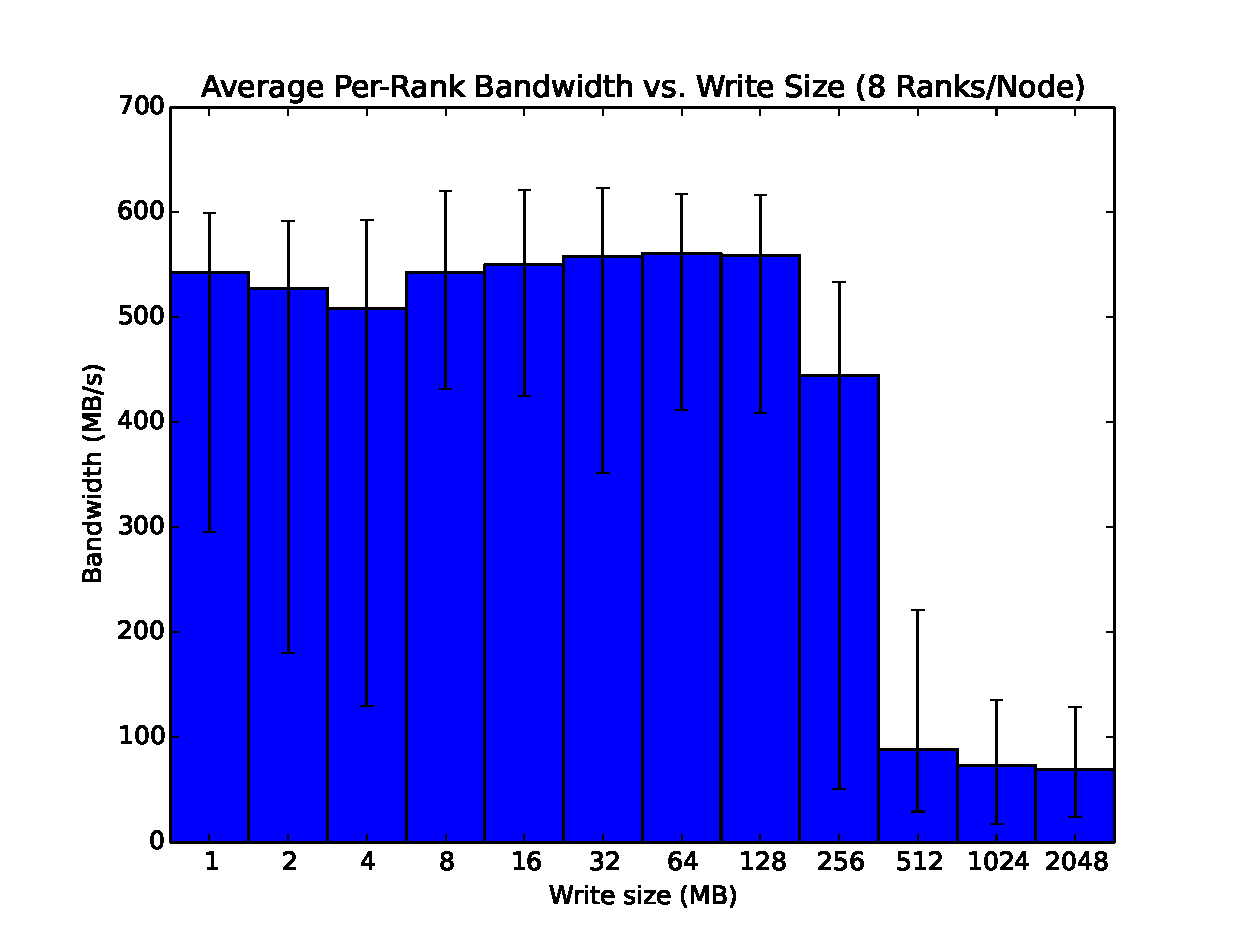
\includegraphics[width=\linewidth]{figures/figure_1.eps}
\caption{Average per-rank write bandwidth using standard \texttt{write()} calls.  8 ranks per node. No GPU memory cache.} 
\label{fig:results_base_8}
\end{figure}

Figure \ref{fig:results_base_8} shows the results of a baseline test.  The colored bars show the average values and the error bars display the minimum and maximum values.  In this test, the application wrote to the filesystem with standard \texttt{write()} calls and the GPU memory was not used at all.\footnote{The daemon process was not even started for this test.}  The results provide some baseline numbers that can be used for comparison with the tests using GPU memory.

Note the sharp drop in performance between 256MB and 512MB.  On Titan, the Lustre client is configured to allow a maximum of 64MB per OST and to default to using 4 OST's per file.  Given the number of OST's available, it's statistically likely that no two output files in this test used the same OST's.  In short, write sizes of 256MB or less were cached in system memory using the existing Lustre client cache and the performance of the 512MB, 1GB and 2GB sizes is dominated by the performance of the filesystem.  In order for this work to be useful, it must obviously improve on that.

\begin{figure}
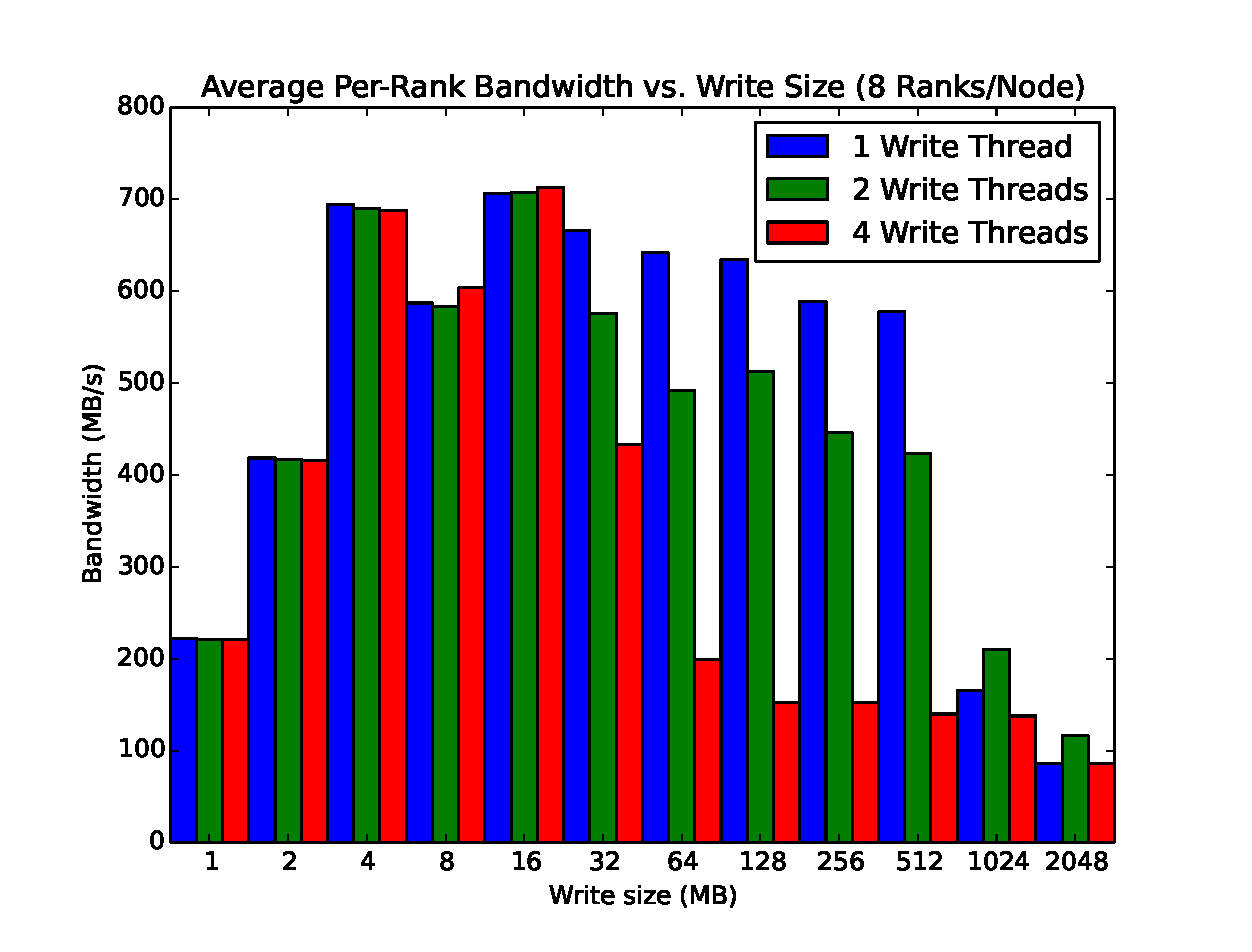
\includegraphics[width=\linewidth]{figures/figure_2.eps}
\caption{Average per-rank write bandwidth.  8 ranks per node.} 
\label{fig:results_8_nobars}
\end{figure}

Figure \ref{fig:results_8_nobars} shows the remaining results of the first test series.  As stated earlier, this series was run with 8 ranks per node and with 1, 2 \& 4 write threads in the daemon.  The graph shows a number of interesting features.  The first and most obvious, is that multiple write threads decrease performance.  Exactly why this is so is unclear, but it appears that having multiple threads read from GPU memory interfered with the individual ranks' ability to copy data into GPU memory.  

Concentrating on the single thread performance, it's clear that the application benefits from using GPU memory out to the 512MB write size.  This makes sense since eight ranks each writing 512MB is a total of 4GB and that will fit into the available GPU memory.  Even at 1GB, the application sees somewhat improved performance because there is enough GPU memory to hold significant fraction of the data to be written.  It's not until the 2GB write size that the write performance is dominated by the filesystem's throughput.

Also obvious from the graph is the fact that small write sizes are not particularly efficient.  For write sizes less than 4MB, copying data to GPU memory is slower than writing to the Lustre cache.  This is not surprising given the results shown in Figure \ref{fig:transfer_bw}.


%\begin{figure}
%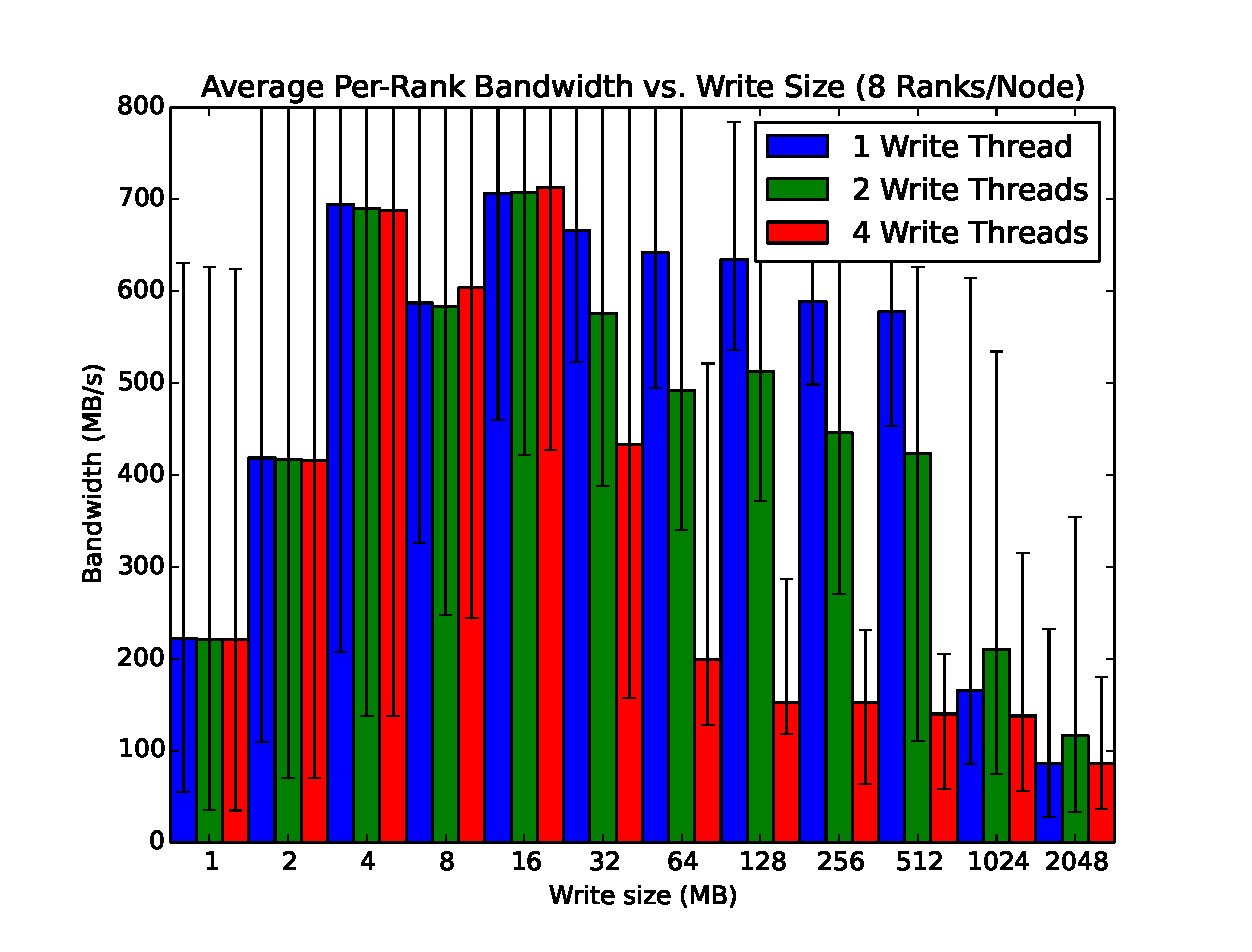
\includegraphics[width=\linewidth]{figures/figure_3.eps}
%\caption{Minimum \& maximum per-rank write bandwidth.  8 ranks per node.} 
%\label{fig:results_8_bars}
%\end{figure}

\begin{figure}
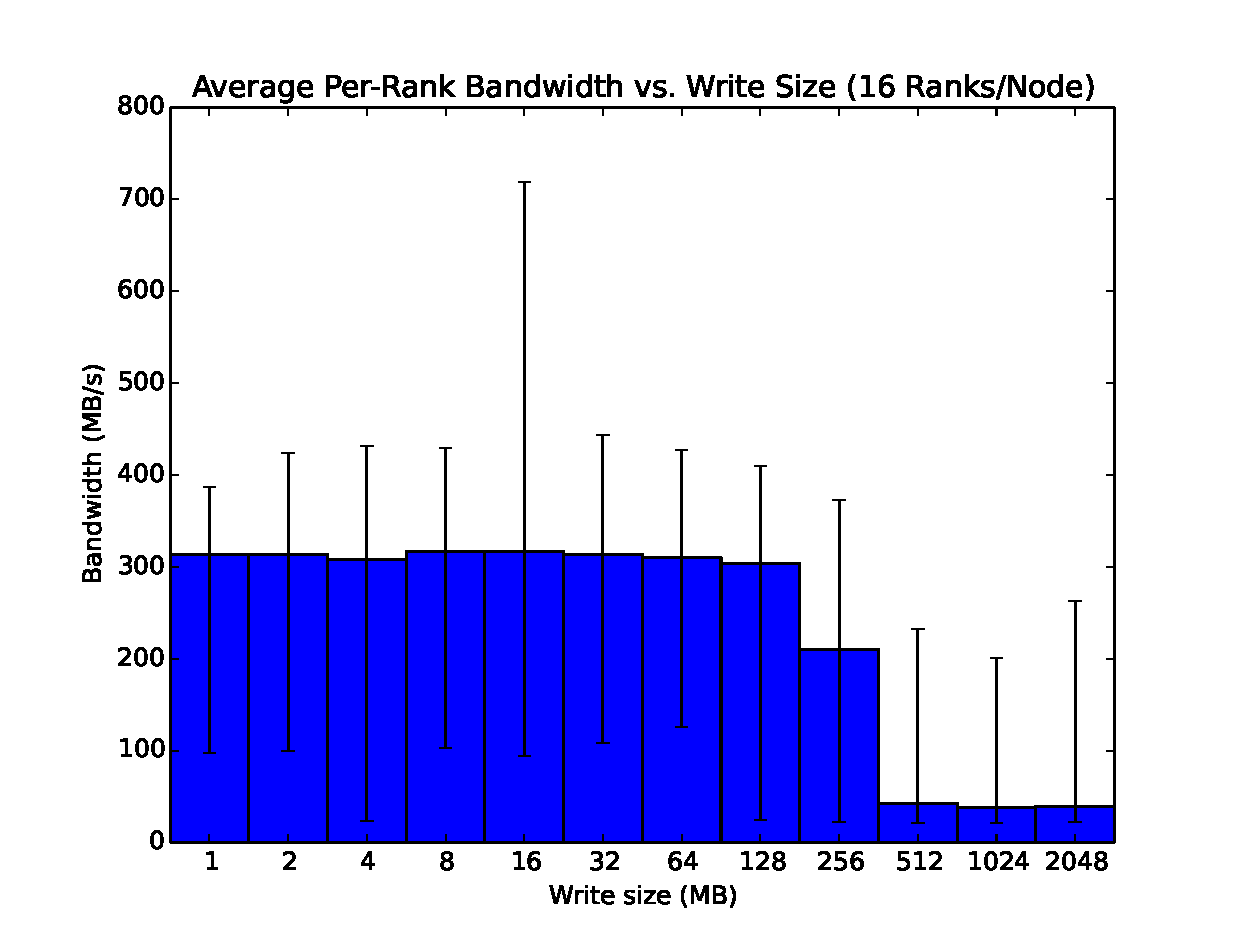
\includegraphics[width=\linewidth]{figures/figure_6.eps}
\caption{Average per-rank write bandwidth using standard \texttt{write()} calls.  16 ranks per node. No GPU memory cache.} 
\label{fig:results_base_16}
\end{figure}

\begin{figure}
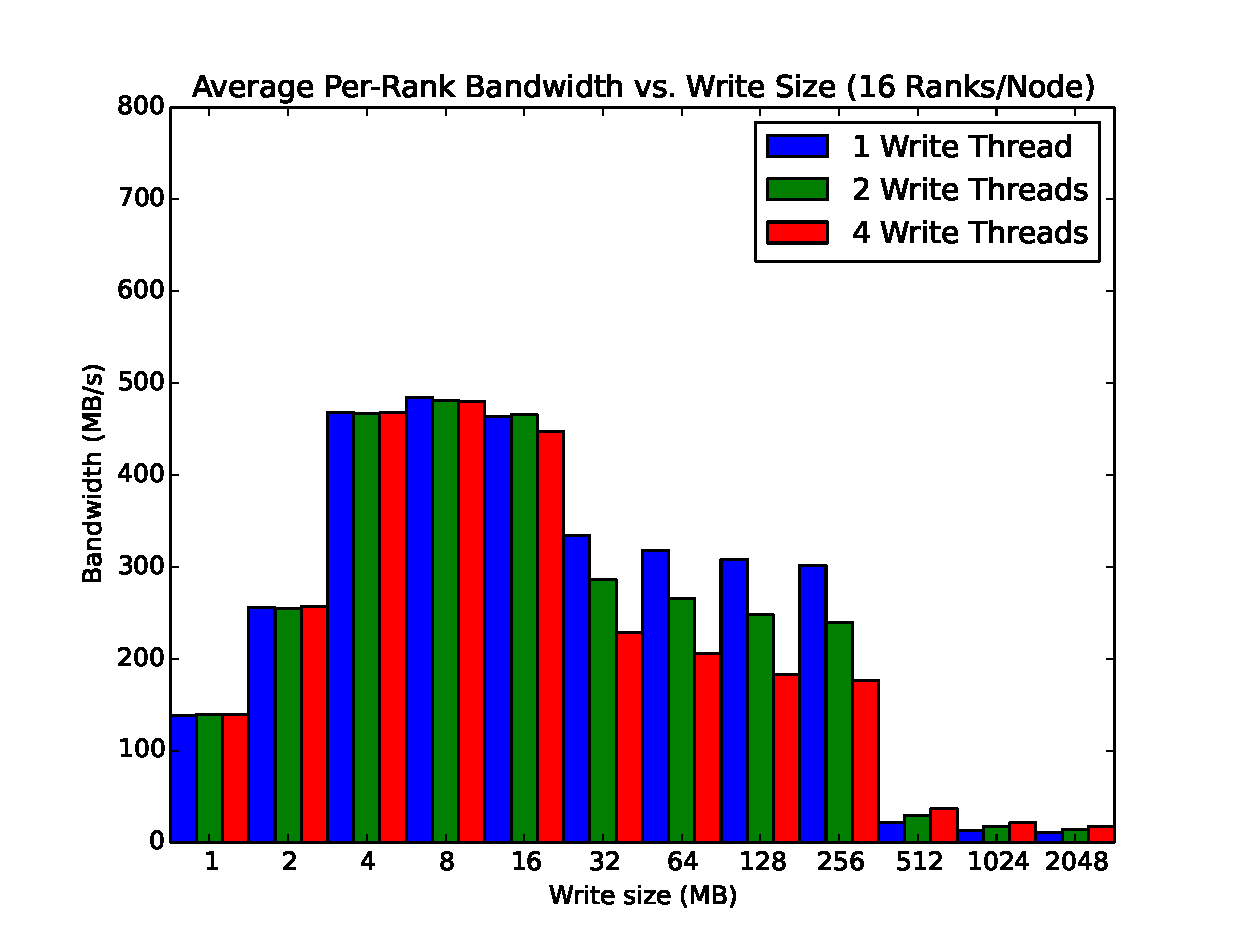
\includegraphics[width=\linewidth]{figures/figure_4.eps}
\caption{Average per-rank write bandwidth.  16 ranks per node.} 
\label{fig:results_16_nobars}
\end{figure}

%\begin{figure}
%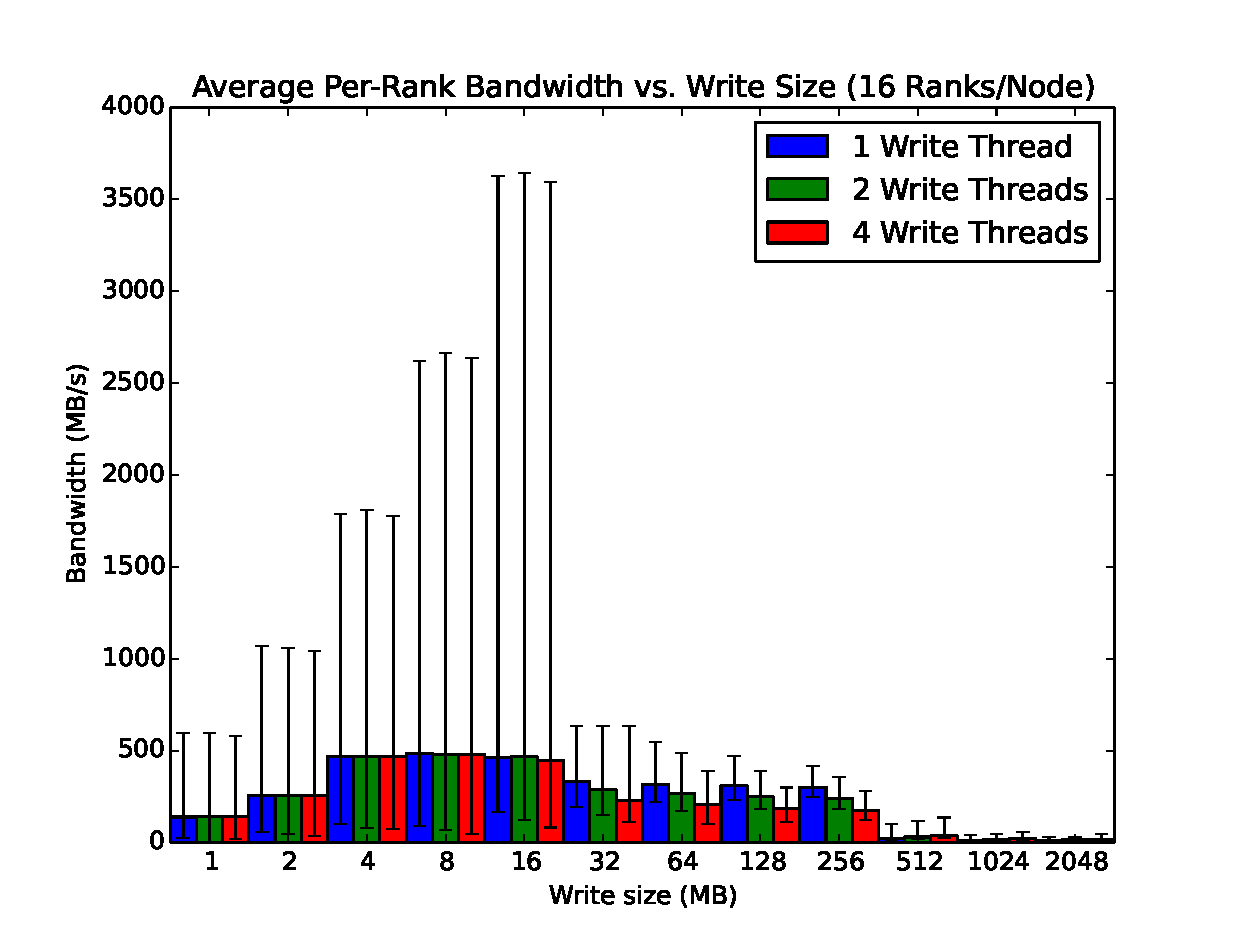
\includegraphics[width=\linewidth]{figures/figure_5.eps}
%\caption{Minimum \& maximum per-rank write bandwidth.  16 ranks per node.} 
%\label{fig:results_16_bars}
%\end{figure}

Figures \ref{fig:results_base_16} and \ref{fig:results_16_nobars} show the results for the second series of tests.  As noted above, this series used 16 ranks per node, plus the daemon's threads.  This meant, of course, that the cores were oversubscribed.  Notice that Figure \ref{fig:results_base_16} has the same basic shape as Figure \ref{fig:results_base_8}.  The only significant difference is that the reported speeds shown in Figure \ref{fig:results_base_16} are approximately half those shown in Figure \ref{fig:results_base_8}.  This is expected, since there are twice as many ranks writing.

Figure \ref{fig:results_16_nobars} shows that again, the per-rank bandwidth is about half that shown in Figure \ref{fig:results_8_nobars} because there are twice as many ranks.  It's also clear that the application ranks see good write performance up to the 256MB write size, which is the largest size that will entirely fit into GPU memory.  It's also clear that, as in the first test series, writes must be at least 4MB in order to get reasonable performance copying the data into GPU memory.


Looking at figure \ref{fig:results_16_nobars}, note the drop in performance between 16MB and 32MB and the slight downward trend from 32MB to 256MB.  This pattern also appears in Figure \ref{fig:results_8_nobars}, but is much more obvious in Figure 
\ref{fig:results_16_nobars}.  The authors hypothesize that this is related to the response time of the daemon.  As mentioned earlier, the daemon allocates GPU memory in blocks of up to 16MB.  Thus, if one of the ranks wants to write more than 16GB, it will need to go through more than one request/response message cycle.  However, the daemon only has a single thread to handle these messages.  When multiple ranks are sending message, they will necessarily have to wait while the daemon services any previous messages and this slows their overall performance.  This is more noticeable in Figure 
\ref{fig:results_16_nobars} because there are more ranks making requests.
In short, it appears that improving the response time of the message handling thread would be beneficial.

\section{Future Work}
\label{sec:future}

Discuss work yet to be done:  add support for caching in system memory,  make 'production ready' (ie: easier for applications to use)
\section{Conclusion}
\label{sec:conclusion}

\todo[inline]{Discuss what we learned; summarize}



% use section* for acknowledgement
\section*{Acknowledgment}
This work was supported by the Oak Ridge Leadership Computing Facility at the Oak Ridge National Laboratory, which is managed by UT Battelle, LLC for the U.S. DOE (under the contract No. DE-AC05-00OR22725).

% conference papers do not normally have an appendix

% trigger a \newpage just before the given reference
% number - used to balance the columns on the last page
% adjust value as needed - may need to be readjusted if
% the document is modified later
%\IEEEtriggeratref{8}
% The "triggered" command can be changed if desired:
%\IEEEtriggercmd{\enlargethispage{-5in}}

% references section

% can use a bibliography generated by BibTeX as a .bbl file
% BibTeX documentation can be easily obtained at:
% http://www.ctan.org/tex-archive/biblio/bibtex/contrib/doc/
% The IEEEtran BibTeX style support page is at:
% http://www.michaelshell.org/tex/ieeetran/bibtex/
%\bibliographystyle{IEEEtran}
% argument is your BibTeX string definitions and bibliography database(s)
%\bibliography{IEEEabrv,../bib/paper}
%
% <OR> manually copy in the resultant .bbl file
% set second argument of \begin to the number of references
% (used to reserve space for the reference number labels box)
\bstctlcite{bstctl:etal, bstctl:nodash, bstctl:simpurl}
\bibliographystyle{IEEEtranS}
\bibliography{references}

\todo[inline]{Double-check the URL for the OA Report - it was giving a 404 error earlier.}


%\begin{thebibliography}{1}
%
%\bibitem{IEEEhowto:kopka}
%H.~Kopka and P.~W. Daly, \emph{A Guide to \LaTeX}, 3rd~ed.\hskip 1em plus
%  0.5em minus 0.4em\relax Harlow, England: Addison-Wesley, 1999.
%
%\end{thebibliography}




% that's all folks
\end{document}



% An example of a floating figure using the graphicx package.
% Note that \label must occur AFTER (or within) \caption.
% For figures, \caption should occur after the \includegraphics.
% Note that IEEEtran v1.7 and later has special internal code that
% is designed to preserve the operation of \label within \caption
% even when the captionsoff option is in effect. However, because
% of issues like this, it may be the safest practice to put all your
% \label just after \caption rather than within \caption{}.
%
% Reminder: the "draftcls" or "draftclsnofoot", not "draft", class
% option should be used if it is desired that the figures are to be
% displayed while in draft mode.
%
%\begin{figure}[!t]
%\centering
%\includegraphics[width=2.5in]{myfigure}
% where an .eps filename suffix will be assumed under latex, 
% and a .pdf suffix will be assumed for pdflatex; or what has been declared
% via \DeclareGraphicsExtensions.
%\caption{Simulation Results}
%\label{fig_sim}
%\end{figure}

% Note that IEEE typically puts floats only at the top, even when this
% results in a large percentage of a column being occupied by floats.


% An example of a double column floating figure using two subfigures.
% (The subfig.sty package must be loaded for this to work.)
% The subfigure \label commands are set within each subfloat command, the
% \label for the overall figure must come after \caption.
% \hfil must be used as a separator to get equal spacing.
% The subfigure.sty package works much the same way, except \subfigure is
% used instead of \subfloat.
%
%\begin{figure*}[!t]
%\centerline{\subfloat[Case I]\includegraphics[width=2.5in]{subfigcase1}%
%\label{fig_first_case}}
%\hfil
%\subfloat[Case II]{\includegraphics[width=2.5in]{subfigcase2}%
%\label{fig_second_case}}}
%\caption{Simulation results}
%\label{fig_sim}
%\end{figure*}
%
% Note that often IEEE papers with subfigures do not employ subfigure
% captions (using the optional argument to \subfloat), but instead will
% reference/describe all of them (a), (b), etc., within the main caption.


% An example of a floating table. Note that, for IEEE style tables, the 
% \caption command should come BEFORE the table. Table text will default to
% \footnotesize as IEEE normally uses this smaller font for tables.
% The \label must come after \caption as always.
%
%\begin{table}[!t]
%% increase table row spacing, adjust to taste
%\renewcommand{\arraystretch}{1.3}
% if using array.sty, it might be a good idea to tweak the value of
% \extrarowheight as needed to properly center the text within the cells
%\caption{An Example of a Table}
%\label{table_example}
%\centering
%% Some packages, such as MDW tools, offer better commands for making tables
%% than the plain LaTeX2e tabular which is used here.
%\begin{tabular}{|c||c|}
%\hline
%One & Two\\
%\hline
%Three & Four\\
%\hline
%\end{tabular}
%\end{table}


% Note that IEEE does not put floats in the very first column - or typically
% anywhere on the first page for that matter. Also, in-text middle ("here")
% positioning is not used. Most IEEE journals/conferences use top floats
% exclusively. Note that, LaTeX2e, unlike IEEE journals/conferences, places
% footnotes above bottom floats. This can be corrected via the \fnbelowfloat
% command of the stfloats package.





